%%%%%%%%%%%%%%%%%%%%%%%%%%%%%%%%%%%%%%%%%%%%%%%%%%%%%%%%
%%%%                                              %%%%%%
%%%%  Author: Peter Wilson                        %%%%%%
%%%%                                              %%%%%%
%%%%  Composite shells                        %%%%%%
%%%%                                              %%%%%%
%%%%%%%%%%%%%%%%%%%%%%%%%%%%%%%%%%%%%%%%%%%%%%%%%%%%%%%%


%fref generates automatically the respective abreviation/word in the text for the reference. You just have to define a label starting with the respective keyword.
%english: chap, sec, fig, eq, app
%deutsch: chap/kap, abs, abb, gl, anh
%see http://ctan.space-pro.be/tex-archive/macros/latex/contrib/fancyref/fancyref.pdf for more \section

%\onehalfspacing
%\setlength{\belowcaptionskip}{-17pt}

\chapter{Extension of shells to composite laminates}
\label{chap:chapter_composite_formulation_implementation}

\renewcommand{\Thema}{Extension of shells to composite laminates}

\lettrine[lines=2]{W}{ith} the ANDES-DKQ and DSG elements formulated and implemented for isotropic materials in the preceding chapters, extending them into composite laminate materials is now considered. The relevant theory is covered in chapter \ref{chap:chapter_2_1} which defines the scope of the formulation and implementation discussed here.

\section{Formulation}
The formulation of orthotropic laminate composite is developed further by recalling the continuous form presented in chapter \ref{chap:chapter_2_1} and then transferring this into a discrete and numerically integrable form suitable for programming.

The general laminate shell stress resultants are related via the total combined constitutive matrix $\bar{\mathbf{C}}$ as follows:

\begin{equation} 
\bar{\mathbf{N}} = \bar{\mathbf{C}} \bar{\boldsymbol{\epsilon}} =
\begin{pmatrix}
N_{xx} \\
N_{yy} \\
N_{xy} \\
M_{xx} \\
M_{yy} \\
M_{xy} \\
Q_{x} \\
Q_{y} 
\end{pmatrix} 
=
\begin{pmatrix}
\mathbf{A} & \mathbf{B} & \mathbf{0} \\
\mathbf{B} & \mathbf{D} & \mathbf{0} \\
\mathbf{0}& \mathbf{0} & \alpha		\begin{pmatrix}
{A}_{44} & {A}_{45} \\
{A}_{45} & {A}_{55} 
\end{pmatrix} 
\end{pmatrix} 
\begin{pmatrix}
\epsilon_{xx} \\
\epsilon_{yy} \\
2\epsilon_{xy}\\
\kappa_{xx}\\
\kappa_{yy}\\
2\kappa_{xy} \\
2\epsilon_{yz} \\
2\epsilon_{xz}
\end{pmatrix}
\label{eqscomp_laminate_form1}
\end{equation}

The individual entries of the material sub matrices $\mathbf{A},\ \mathbf{B}$ and $\mathbf{C}$ are also recalled:

\begin{equation} 
A_{ij} = 
\int_{\frac{-h}{2}}^{\frac{h}{2}}
\bar{Q}_{ij}
\ dz\ ,
\hspace{5mm}
B_{ij} = 
\int_{\frac{-h}{2}}^{\frac{h}{2}}
\bar{Q}_{ij}\ z
\ dz\ ,
\hspace{5mm}
D_{ij} = 
\int_{\frac{-h}{2}}^{\frac{h}{2}}
\bar{Q}_{ij}\ z^2
\ dz
\label{eqscomp_laminate_form2}
\end{equation}


The entries $\bar{Q}_{ij}^{(k)}$ are rotated lamina stiffness's as per equation \ref{eqscomp_plane_stress_tensor_rotated}, related to the pure lamina-aligned stiffness's through the transformation matrix $\mathbf{T}$ of equation \ref{eqscomp11}.

By shifting perspective from abstract formulation to a calculable approach, the total combined constitutive matrix $\bar{\mathbf{C}}$ of a laminate with $n$ laminae and total thickness $h$ can be decomposed into lamina contributions. Furthermore, the rotation of the lamina stiffness's can be postponed until each lamina constitutive matrix is assembled:

\begin{equation} 
 \bar{\mathbf{C}} = \sum_{k=1}^{n}  \mathbf{T}^{T(k)} {\mathbf{C}}^{(k)}  \mathbf{T}^{(k)}
\label{eqscomp_laminate_form3}
\end{equation}

The integral limits of the material sub matrices, for each lamina $k$, are updated accordingly:

\begin{equation} 
A_{ij}^{(k)} = 
\int_{z_k}^{z_{k+1}}
{Q}_{ij}^{(k)}
\ dz\ ,
\hspace{5mm}
B_{ij}^{(k)} = 
\int_{z_k}^{z_{k+1}}
{Q}_{ij}^{(k)}\ z
\ dz\ ,
\hspace{5mm}
D_{ij}^{(k)} = 
\int_{z_k}^{z_{k+1}}
{Q}_{ij}^{(k)}\ z^2
\ dz
\label{eqscomp_laminate_form4}
\end{equation} 

\section{Implementation}
The general approach of extending both shell elements to composite laminate materials in a sensible and efficient manner was to abstract the composite specifics from the individual element formulation level as much as possible. This was achieved by modifying the existing \texttt{ShellCrossSection} class and adding a new constitutive law class \texttt{LinearElasticOrthotropic2DLaw}. The generalized workflow of both elements is outlined in the following flowchart, highlighting only methods relevant to composites:

\begin{figure}[H]
	% Define block styles
	\tikzstyle{virtual} = [rectangle, minimum width=3cm, minimum height=1cm, text centered, draw=black, fill=orange!30]
	\tikzstyle{process} = [rectangle, minimum width=3cm, minimum height=1cm, text centered, draw=black, fill=white!30]
	\tikzstyle{arrow} = [thick,->,>=stealth]
	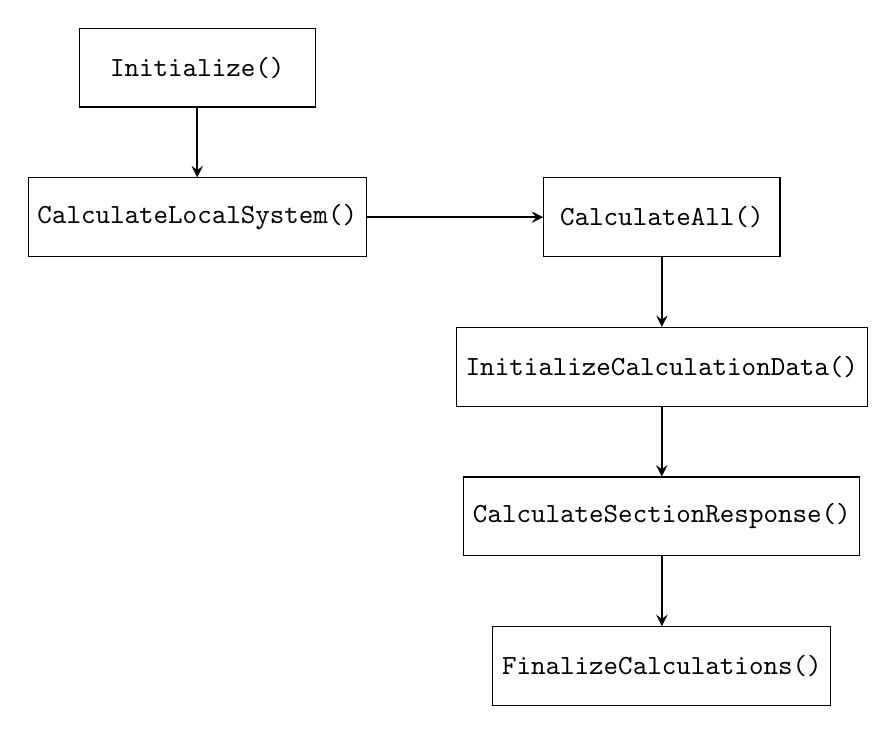
\begin{tikzpicture}[node distance = 1.9cm, auto]
	% Place nodes
	\node [process] (Initialize) {$\texttt{Initialize()}$};
	\node [process, below of=Initialize] (CalculateLocalSystem) {$\texttt{CalculateLocalSystem()}$};
	\node [process, right of=CalculateLocalSystem, xshift = 4cm] (CalculateAll) {$\texttt{CalculateAll()}$};
	\node [process, below of=CalculateAll, xshift = -0cm] (InitializeCalculationData) {$\texttt{InitializeCalculationData()}$};
	\node [process, below of=InitializeCalculationData, yshift = -0cm] (CalculateSectionResponse) {$\texttt{CalculateSectionResponse()}$};
	\node [process, below of=CalculateSectionResponse, yshift = -0cm] (FinalizeCalculations) {$\texttt{FinalizeCalculations()}$};
	% Draw edges
	\draw [arrow] (Initialize) -- (CalculateLocalSystem);
	\draw [arrow] (CalculateLocalSystem) -- (CalculateAll);
	\draw [arrow] (CalculateAll) -- (InitializeCalculationData);
	\draw [arrow] (InitializeCalculationData) -- (CalculateSectionResponse);
	\draw [arrow] (CalculateSectionResponse) -- (FinalizeCalculations);
	\end{tikzpicture}
	\caption{High level overview of composite element workflow}
	\label{compositeworkflow}
\end{figure}

Focussing on calculate section response():

\begin{figure}[H]
	% Define block styles
	\tikzstyle{virtual} = [rectangle, minimum width=3cm, minimum height=1cm, text centered, draw=black, fill=orange!30]
	\tikzstyle{process} = [rectangle, minimum width=3cm, minimum height=1cm, text centered, draw=black, fill=white!30]
	\tikzstyle{arrow} = [thick,->,>=stealth]
	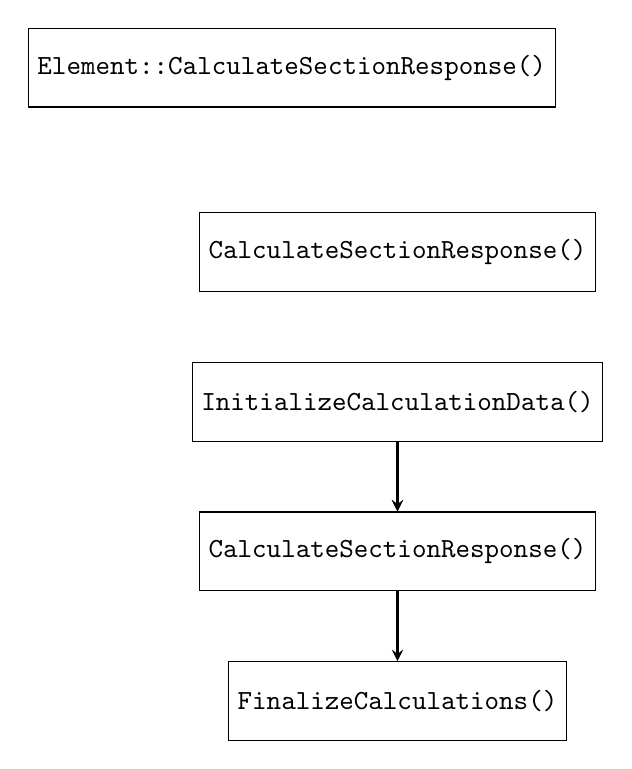
\begin{tikzpicture}[node distance = 1.9cm, auto]
	% Place nodes
	\node [process] (Element::CalculateSectionResponse) {$\texttt{Element::CalculateSectionResponse()}$};
	\node [process, below right of=Element::CalculateSectionResponse, xshift = 0cm, yshift = -1cm] (CalculateSectionResponse) {$\texttt{CalculateSectionResponse()}$};
	\node [process, below of=CalculateSectionResponse, xshift = -0cm] (InitializeCalculationData) {$\texttt{InitializeCalculationData()}$};
	\node [process, below of=InitializeCalculationData, yshift = -0cm] (CalculateSectionResponse) {$\texttt{CalculateSectionResponse()}$};
	\node [process, below of=CalculateSectionResponse, yshift = -0cm] (FinalizeCalculations) {$\texttt{FinalizeCalculations()}$};
	% Draw edges
	\draw [arrow] (InitializeCalculationData) -- (CalculateSectionResponse);
	\draw [arrow] (InitializeCalculationData) -- (CalculateSectionResponse);
	\draw [arrow] (CalculateSectionResponse) -- (FinalizeCalculations);
	\end{tikzpicture}
	\caption{High level overview of composite element workflow scoped to ShellCrossSection}
	\label{compositeworkflow2}
\end{figure}



asdfdsf


\begin{algorithm}
	\onehalfspacing
	\caption{Generalized composite shell element stiffness matrix pseudocode}\label{general composite shell pseudocode}
	\begin{algorithmic}[1]
		\Require Orthotropic laminate material data specified
		\State \textbf{call} $\texttt{Initialize()}$
		\State \hspace{\algorithmicindent}\textbf{if} $materialProperties$ has orthotropic laminate data \textbf{then}
		\State \hspace{\algorithmicindent} \hspace{\algorithmicindent} Create and assign $\texttt{LinearElasticOrthotropic2DLaw}$
		\State \hspace{\algorithmicindent} \hspace{\algorithmicindent} Parse composite material data in $\texttt{ShellCrossSection}$
		\State \hspace{\algorithmicindent}\textbf{end if}
		\State \textbf{call} $\texttt{CalculateAll()}$
		\State \hspace{\algorithmicindent}Perform element-specific calculations (may enter Gauss loop)
		\State \hspace{\algorithmicindent}\textbf{call} $\texttt{CalculateSectionResponse}()$
		\State \hspace{\algorithmicindent}\hspace{\algorithmicindent} \textbf{call} $\texttt{ShellCrossSection::CalculateSectionResponse}()$
		\State \hspace{\algorithmicindent} \hspace{\algorithmicindent} \hspace{\algorithmicindent} \textbf{while} ($k$ < number of laminae) \textbf{do}
		\State \hspace{\algorithmicindent} \hspace{\algorithmicindent} \hspace{\algorithmicindent} \hspace{\algorithmicindent}Retrieve stiffnesses of $k^{th}$ lamina $\mathbf{Q}^{(k)}$ from material law
		\State \hspace{\algorithmicindent} \hspace{\algorithmicindent} \hspace{\algorithmicindent} \hspace{\algorithmicindent}Assemble and integrate unrotated lamina constitutive matrix $\mathbf{C}^{(k)}$
		\State \hspace{\algorithmicindent} \hspace{\algorithmicindent} \hspace{\algorithmicindent} \hspace{\algorithmicindent}\textbf{if} $laminaOrientationAngle \neq 0$ \textbf{then}
		\State \hspace{\algorithmicindent} \hspace{\algorithmicindent} \hspace{\algorithmicindent} \hspace{\algorithmicindent} \hspace{\algorithmicindent} Transform $\mathbf{C}^{(k)}$ into $\bar{\mathbf{C}}^{(k)}$
		\State \hspace{\algorithmicindent} \hspace{\algorithmicindent} \hspace{\algorithmicindent} \hspace{\algorithmicindent}\textbf{end if}
		\State \hspace{\algorithmicindent} \hspace{\algorithmicindent} \hspace{\algorithmicindent} \hspace{\algorithmicindent}Add lamina $\bar{\mathbf{C}}^{(k)}$ to laminate $\bar{\mathbf{C}}$
		\State \hspace{\algorithmicindent} \hspace{\algorithmicindent} \hspace{\algorithmicindent} \textbf{end while}
		\State \hspace{\algorithmicindent}Assemble element-specific stiffness matrix and finalize calculations
	\end{algorithmic}
\end{algorithm}



asdfadsf


\begin{algorithm}
	\onehalfspacing
	\caption{Generalized composite shell element stress and strain recovery}
	\label{general composite shell stress pseudocode}
	\begin{algorithmic}[1]
		\Require $requestedQuantity = laminateStresses$, calculation of nodal displacements
		\State Perform all preliminary operations necessary to determine mid-plane $generalizedStrains$
		\While{Gauss loop}
		\State \textbf{call} $\texttt{CalculateGaussPointContribution}(data)$
		\State \hspace{\algorithmicindent}\textbf{call} $\texttt{CalculateBMatrix}(data)$
		\State \hspace{\algorithmicindent}\hspace{\algorithmicindent} Calculate combined $B$ at current $gaussPoint$
		\State $generalizedStrains$ = product$(B,\ localDisplacements)$
		\State \textbf{call} $\texttt{CalculateLaminaStrains}(data)$
		\State \hspace{\algorithmicindent}Determine $laminateStrains$ at top and bottom surface of each lamina 
		\State \textbf{call} $\texttt{CalculateLaminaStresses}(data)$
		\State \hspace{\algorithmicindent}Retrieve raw laminae stiffnesses
		\State \hspace{\algorithmicindent}\textbf{while} ($k$ < number of laminae) \textbf{do}
		\State \hspace{\algorithmicindent} \hspace{\algorithmicindent}$laminateStresses^{(2k)}$ = product$(\mathbf{C}^{(2k)},\ laminateStrains^{(2k)})$
		\State \hspace{\algorithmicindent} \hspace{\algorithmicindent}$laminateStresses^{(2k+1)}$ = product$(\mathbf{C}^{(2k+1)},\ laminateStrains^{(2k+1)})$
		\State \hspace{\algorithmicindent}\textbf{while end}
		\If{$laminateStresses$ requires local orientation} 
		\State Rotate $laminateStresses$ to local orientation
		\EndIf
		\State Assemble $laminateStresses$ into $outputMatrix$
		\If{$laminateStresses$ requires global orientation} 
		\State Rotate $outputMatrix$ to global orientation
		\EndIf
		\State Interpolate $outputMatrix$ to standard Gauss points for visualisation
		\EndWhile
	\end{algorithmic}
\end{algorithm}